\chapter{The project}
\label{chap:the_project}

\section{Ground station networks}

The actual performance of any future network will depend on the participants, their location and hardware. All of this is currently unknown. In \autoref{fig:ground_networks} and \autoref{tab:networks} some different networks are illustrated and their access time simulated.

\begin{figure}
\begin{subfigure}{.5\textwidth}
	\centering
	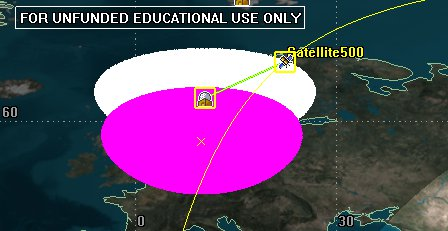
\includegraphics[width=\textwidth]{Figures/range_ntnu_aalborg}
	\label{fig:range_ntnu_aalborg}
\end{subfigure}
\begin{subfigure}{.5\textwidth}
	\centering
	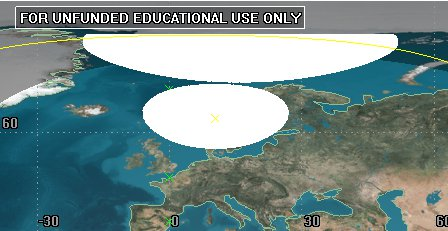
\includegraphics[width=\textwidth]{Figures/range_ntnu_svalbard}
	\label{fig:range_ntnu_unis}
\end{subfigure}
\begin{subfigure}{.5\textwidth}
	\centering
	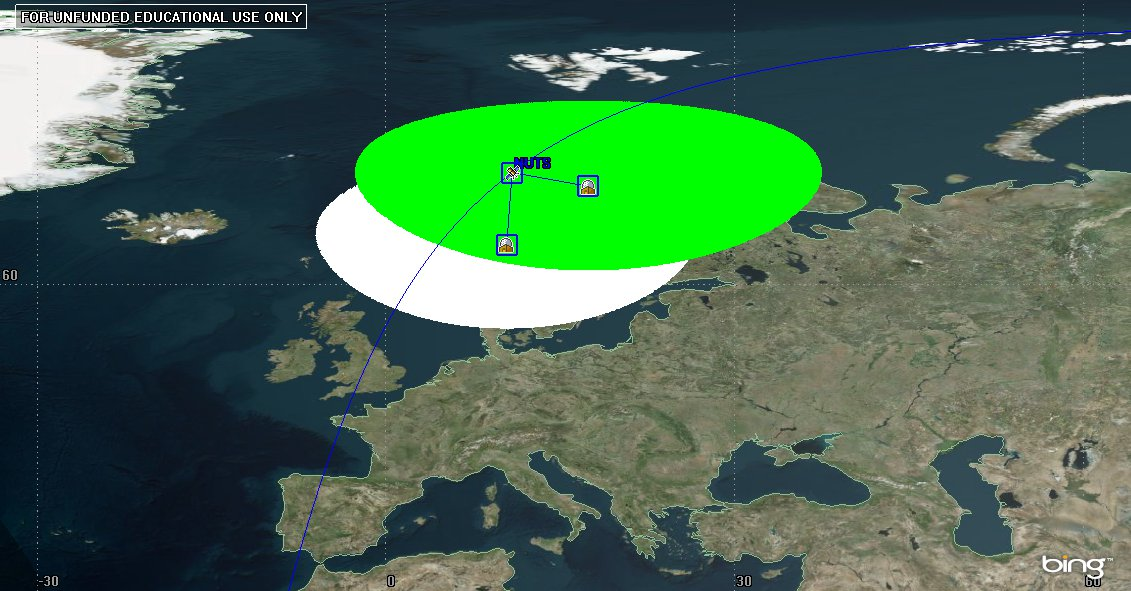
\includegraphics[width=\textwidth]{Figures/range_ntnu_narvik}
	\label{fig:range_ntnu_narvik}
\end{subfigure}
\begin{subfigure}{.5\textwidth}
	\centering
	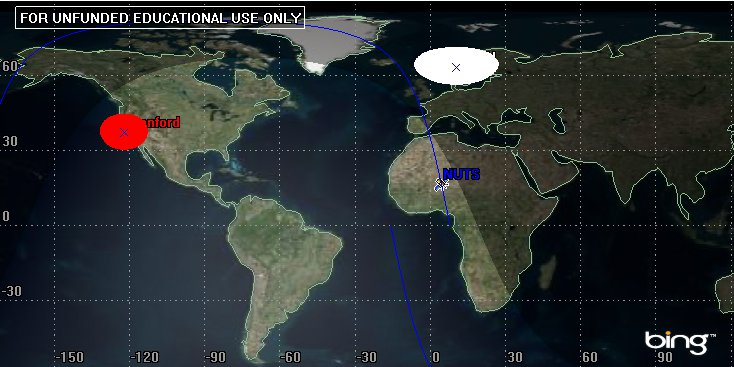
\includegraphics[width=\textwidth]{Figures/range_ntnu_stanford}
	\label{fig:range_ntnu_narvik}
\end{subfigure}
\caption{Some possible ground networks}
\label{fig:ground_networks}
\end{figure}

\begin{table}
	\begin{center}
	\begin{tabular}{l | c c}
  	Other locations & Time & Improvement \\
	\hline \hline
	Aalborg & 790s &  50\% \\
	\hline
	Longyearbyen & 1900s & 260\% \\
	\hline
	Narvik & 900s & 73\%  \\
	\hline
	Stanford & 800s & 54\% 
	\end{tabular}
	\end{center}
	\caption{Results of simulations}
	\label{tab:networks}
\end{table}

These results show that even cooperating with other norwegian/scandinavian universities will result in significant gains in download capacity, even though there will be a certain overlap in coverage. Cooperating with other universities further afield will also increase download capacity, but if they are located at lower latitudes the decreased number of passes observed will decrease their contribution.  

\section {The project}

The problem today is that the transfer antenna on the NUTS satellite is limited. We started looking for a network that connects ground stations to Internet. From there we wanted a ground station that was portable and easy to use (plug and play). We therefore decided to try out Raspberry Pi.

\section {Software}

The first thing we had to do was to install the Carpcomm software. We installed the CarpSD ground station control software. This is an open-source program primarily developed by the team behind Carpcomm. The purpose of this software is to make it possible to connect to the Carpcomm server. It also makes it possible to control the ground station if you have access to a web-browser. This is possible because the software runs a background process on the Raspberry Pi. The software runs continuously in the background making is possible to connect to at any time and start receiving from satellites. 

The next thing we had to do was to create a entry for our station plotting the latitude, longitude and elevation.    
Since the Raspberry didn’t have a connector for the box that controls the antenna we had to make a cable so we could get the two components to communicate. (image) 
We had some troubles with this cable because it wasn't robust enough. We thought about making a new one, but we didn't have the time for it. 
The last thing we had to do before we could start testing was to install the software for the antenna controller. We installed the Hamlib rotator library since it was supported by our rotator. 

Now everything was set to start testing the station. We started of with connecting a small TV-antenna to see if we got a signal. On the station page at the Carpcomm website we tuned it to 433.3 MHz. The reason for this  frequency is because its used by the police in Trondheim and there are likely to be a lot of transmissions there.  We managed to receive data and publish it to the Carpcomm network.

\begin{figure}
\begin{subfigure}{.5\textwidth}
	\centering
	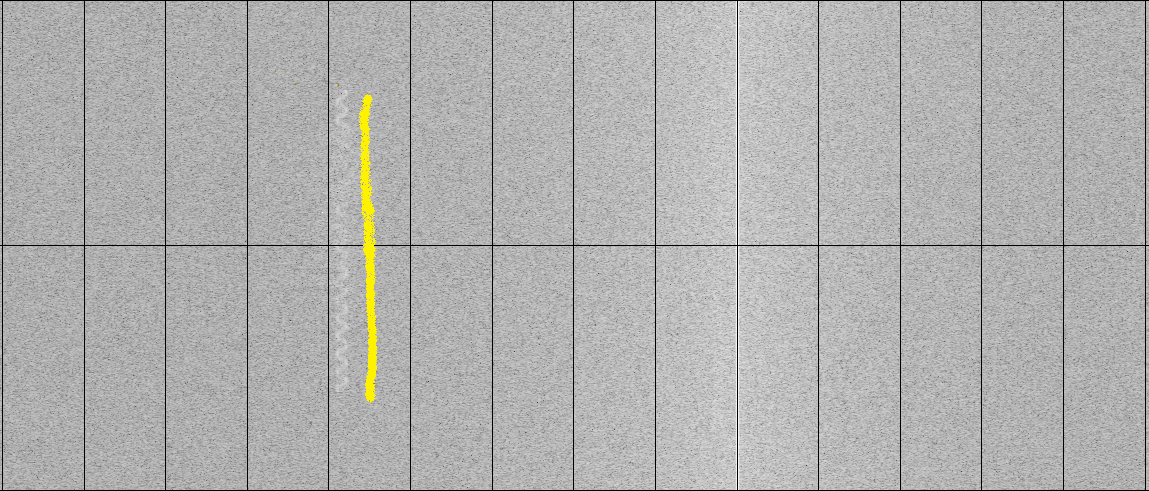
\includegraphics[width=\textwidth]{Figures/sattelite_transmition}
	\label{fig: Transmission}
\end{subfigure}
\end{figure}
A short explanation of the recorded transmission. The x-axis is the frequency and the y-axis it time. Black and gray is noise and the white left of the yellow line is signals.  

 Next stop was to try with a full scale antenna. We succeed in receiving data but we could not get the antenna rotor to work. So this remains unsolved. Another problem is that the Carpcomm software only supports retrieving data, not send. So if the satellite does not send by themselves we have no way of telling it to start transmitting. 




